\documentclass[10pt]{article}
\usepackage[T1]{fontenc}
\usepackage{lmodern}
\usepackage[margin=1in]{geometry}
\usepackage{amsmath,amssymb,amsthm}
\usepackage{graphicx}
\usepackage{microtype}
\usepackage[hidelinks]{hyperref}
\hypersetup{pdftitle={Average precision under random ranking: baseline, variability, and formal verification},pdfauthor={Shantanu Singh and Anne E. Carpenter}}
\newtheorem{proposition}{Proposition}
\newtheorem{corollary}{Corollary}
\newcommand{\E}{\mathbb{E}}
\newcommand{\Var}{\operatorname{Var}}
\newcommand{\AP}{\operatorname{AP}}
\title{Average precision under random ranking:\\baseline, variability, and formal verification}
\author{Shantanu Singh \and Anne E. Carpenter}
\makeatletter
\let\originalmaketitle\@maketitle
\def\@maketitle{\originalmaketitle\vspace{-1.5em}\begin{center}
Broad Institute of MIT and Harvard\\
\small\href{mailto:shantanu@broadinstitute.org}{shantanu@broadinstitute.org}\quad
\href{mailto:anne@broadinstitute.org}{anne@broadinstitute.org}
\end{center}}
\makeatother
\date{September 7, 2026}
\begin{document}
\maketitle
\begin{abstract}
Average precision under random ranking depends on both the number of relevant items and the list length.
Its expectation exceeds prevalence when relevant and irrelevant items are both present.
We give a short derivation of the harmonic expectation and organize the second moment into four sums according to the number of distinct ranks in each product.
The resulting expressions recover existing moment results, including the full-ranking specialization of formulas for average precision at a cutoff.
We accompany the derivations with Lean proofs and a deterministic Python demonstration.
Two asymptotic regimes show why fixed prevalence and a fixed number of relevant items give different variance coefficients.
An enumerated example distinguishes compact moment formulas from a representation of the full distribution that still requires counting rank subsets.
\end{abstract}

\section{Introduction}
Average precision (AP) summarizes how early a ranking retrieves relevant items.
Interpreting a score relative to chance requires specifying both a random-ranking model and the quantities being compared.
The null mean describes the baseline, the variance describes fluctuations, and tail probabilities answer a different question.
Confusing these quantities can make a baseline correction appear to provide more statistical information than it does.

Exact AP moment calculations are already available.
Zhang and Su organize the first two moments through hit-rank distributions~\cite{zhang}.
Lopes and Bontempi study the null mean and variance for AP and discuss other precision--recall interpolation rules~\cite{lopes}.
Bestgen provides an exact hypergeometric baseline calculation~\cite{bestgen}.
Manzhos, Ianevych, and Melnyk give harmonic expectation and variance formulas for AP at a cutoff under two sampling models~\cite{manzhos}.
Their sampling-without-replacement model, specialized to the full ranking, gives the same moments as those presented here.

This note provides readable derivations, explicit boundary cases, and accompanying formal verification.
The mean follows by conditioning on the rank of one relevant item.
The second moment follows by classifying products according to the number of distinct ranks involved.
We distinguish these moment formulas from the exact rank-subset representation of the distribution, whose evaluation still requires counting.
We make no first-discovery claim for the moments or their asymptotics.

The harmonic expectation and its exchangeability derivation were recorded in this project's repository in September 2025, before the November 2025 preprint of Manzhos and colleagues.
A complete Lean verification of the expectation was added in March 2026; the variance derivation and verification were added in July 2026.
These dates describe the recorded development history rather than establishing publication priority.
The corresponding commits are identified in the accompanying verification record.

\section{The random-ranking model}
Let a list have length $L$, with exactly $M$ relevant items, where $1\le M\le L$.
Write $Z_k\in\{0,1\}$ for relevance at rank $k$.
Full-list, non-interpolated AP is
\begin{equation}\label{eq:ap}
 A=\frac{1}{M}\sum_{k=1}^{L}\frac{Z_k}{k}\sum_{i=1}^{k}Z_i.
\end{equation}
We assume a uniformly random permutation of the items, conditional on their relevance labels.
The relevant ranks therefore form a uniform size-$M$ subset of $\{1,\ldots,L\}$: each subset has $M!(L-M)!$ permutation preimages.
For ordered relevant ranks $R_1<\cdots<R_M$, equation~\eqref{eq:ap} becomes
\begin{equation}\label{eq:ranks}
 A=\frac{1}{M}\sum_{j=1}^{M}\frac{j}{R_j}.
\end{equation}
The model fixes the positive count; it is not a model of independently sampled relevance indicators.
If scores are tied, a ranking procedure must specify a tie-breaking rule, and the results apply only when its resulting null ranking has the stated uniform law.
For $M=L$, AP is identically one.
We assign AP zero at $M=0$, but the nonzero-positive formulas below do not extend to that case by substituting $M=0$.

\section{The exact baseline}
\begin{proposition}[Expectation]\label{prop:mean}
For $L>1$ and $1\le M\le L$, let $H_L=\sum_{k=1}^L1/k$.
Then
\begin{align}
 \mu_0=\E[A]
 &=\frac1L\left[\frac{M-1}{L-1}(L-H_L)+H_L\right]\label{eq:mean}\\
 &=\frac ML+\frac{(L-M)(H_L-1)}{L(L-1)}.\label{eq:bias}
\end{align}
\end{proposition}
\begin{proof}
Choose one relevant item and denote its rank by $R$.
Its rank is uniform on $\{1,\ldots,L\}$.
Conditional on $R=r$, the expected number of other relevant items before it is $(r-1)(M-1)/(L-1)$.
Its expected precision is therefore
\[
 \frac1r\left[1+\frac{(r-1)(M-1)}{L-1}\right].
\]
By symmetry, every relevant item has the same expected precision, so averaging this expression over $r$ gives $\E[A]$.
The sums of $1/r$ and $(r-1)/r$ are $H_L$ and $L-H_L$, which proves~\eqref{eq:mean}.
Rearrangement gives~\eqref{eq:bias}.
\end{proof}
The correction is strictly positive for $1\le M<L$.
At $L=M=1$, the expectation is one.
For fixed $p=M/L\in(0,1)$ along lists with integer $pL$, the expansion $H_L=\log L+O(1)$ gives
\[
 \mu_0=p+\frac{(1-p)\log L}{L}+O(L^{-1}).
\]
For fixed $M$, however,
\begin{equation}\label{eq:relative}
 \frac{\mu_0}{M/L}=1+\frac{(L-M)(H_L-1)}{M(L-1)}.
\end{equation}
The relative correction grows logarithmically even though both the expectation and prevalence tend to zero.

\subsection{Connection to hit-rank calculations}
The same expectation can be calculated by summing over relevant-item positions.
Choosing $j-1$ positives before rank $k$ and $M-j$ after it gives
\[
 q_{jk}=\Pr(R_j=k)=\frac{\binom{k-1}{j-1}\binom{L-k}{M-j}}{\binom LM},
\]
with inadmissible binomial coefficients interpreted as zero.
For $L>1$, summing over the identity of the positive at rank $k$ gives
\[
 \sum_{j=1}^M j q_{jk}
 =\E\left[Z_k\sum_{i=1}^kZ_i\right]
 =\frac ML+(k-1)\frac{M(M-1)}{L(L-1)}.
\]
Multiplying by $1/(Mk)$ and summing over $k$ recovers Proposition~\ref{prop:mean}.
This identity connects a hit-rank representation to a harmonic evaluation without finding the distribution of AP itself.
The corresponding second-moment approaches likewise average products of the same statistic in different orders.

\section{The second moment}
Write $W=MA$ and define, for positive integers $r$,
\[
 m_r=\begin{cases}\binom Mr/\binom Lr,&r\le M,\\0,&r>M.\end{cases}
\]
For $r\le L$, $m_r$ is the probability that $r$ prescribed distinct ranks are all relevant.
The zero convention also avoids singular formulas when $L<r$.
Write $H=H_L$ and $H_2=\sum_{k=1}^L1/k^2$.
\begin{proposition}[Second moment]\label{prop:second}
For $1\le M\le L$,
\begin{align}
 \E[W]&=m_1H+m_2(L-H),\label{eq:ew}\\
 \E[W^2]&=m_1H_2+m_2(2H^2+3H-5H_2)\notag\\
 &\quad+m_3(2LH+5L-5H^2-9H+7H_2)\notag\\
 &\quad+m_4(L^2-2LH-5L+3H^2+6H-3H_2),\label{eq:ew2}\\
 \Var(A)&=\frac{\E[W^2]-\E[W]^2}{M^2}.\label{eq:var}
\end{align}
\end{proposition}
\begin{proof}
Expand $W=\sum_{i\le k}Z_iZ_k/k$ and its square.
The expected product associated with two index pairs $(i,k)$ and $(j,l)$ is $m_r$, where $r=|\{i,k,j,l\}|$.
The coefficient of $m_r$ is therefore the sum of $1/(kl)$ over ordered pairs of index pairs having union cardinality $r$.
Appendix~\ref{app:sums} evaluates these four coefficients and yields~\eqref{eq:ew2}.
The first moment follows by separating $i=k$ from $i<k$, and~\eqref{eq:var} is the definition of variance.
\end{proof}
For $M=L$, the variance vanishes.
For $M=1$, it is $H_2/L-(H/L)^2$, since AP is the reciprocal of a uniform rank.
The expressions apply at $L=1,2,3$ without dividing by falling factorials that vanish.

Theorem 1 of Manzhos et al.~\cite{manzhos} normalizes AP at cutoff $k$ by $\min(k,m)$ when there are $m$ positives among $N$ items.
Setting $k=N=L$ and $m=M$ gives the normalization in~\eqref{eq:ap}.
Our supplementary symbolic calculation shows that their resulting variance and~\eqref{eq:var} are identical as rational expressions for $L\ge4$.
The smaller lists are covered directly by Proposition~\ref{prop:second}.
For comparison with Lopes and Bontempi~\cite{lopes}, the relevant statistic is their $\mathrm{AUPRC}_{p\mathrm{max}}$; their other interpolation rules define different statistics.

\subsection{Two variance regimes}
\begin{corollary}\label{cor:asymptotic}
For fixed prevalence $p=M/L\in(0,1)$ along lists with integer $pL$,
\[
 \Var(A)=\frac{p(1-p)}{L}+O\left(\frac{\log^2L}{L^2}\right).
\]
For fixed $M\ge1$,
\[
 \Var(A)\sim\frac{\pi^2}{6ML}.
\]
\end{corollary}
Appendix~\ref{app:asymptotic} derives these expansions from Proposition~\ref{prop:second}.
The fixed-prevalence expansion is not uniform down to prevalence zero.
Substituting $p=M/L$ into its leading term while holding $M$ fixed would consequently give the wrong order of variance.

\section{Demonstration and interpretation}
Figure~\ref{fig:demo} displays the baseline correction and the two variance regimes.
The calculations use exact rational moments, converted to floating point only for plotting.
A small distribution is computed independently by enumerating binary label vectors and scoring cumulative precision at relevant ranks.

\begin{figure}[tbp]
\centering
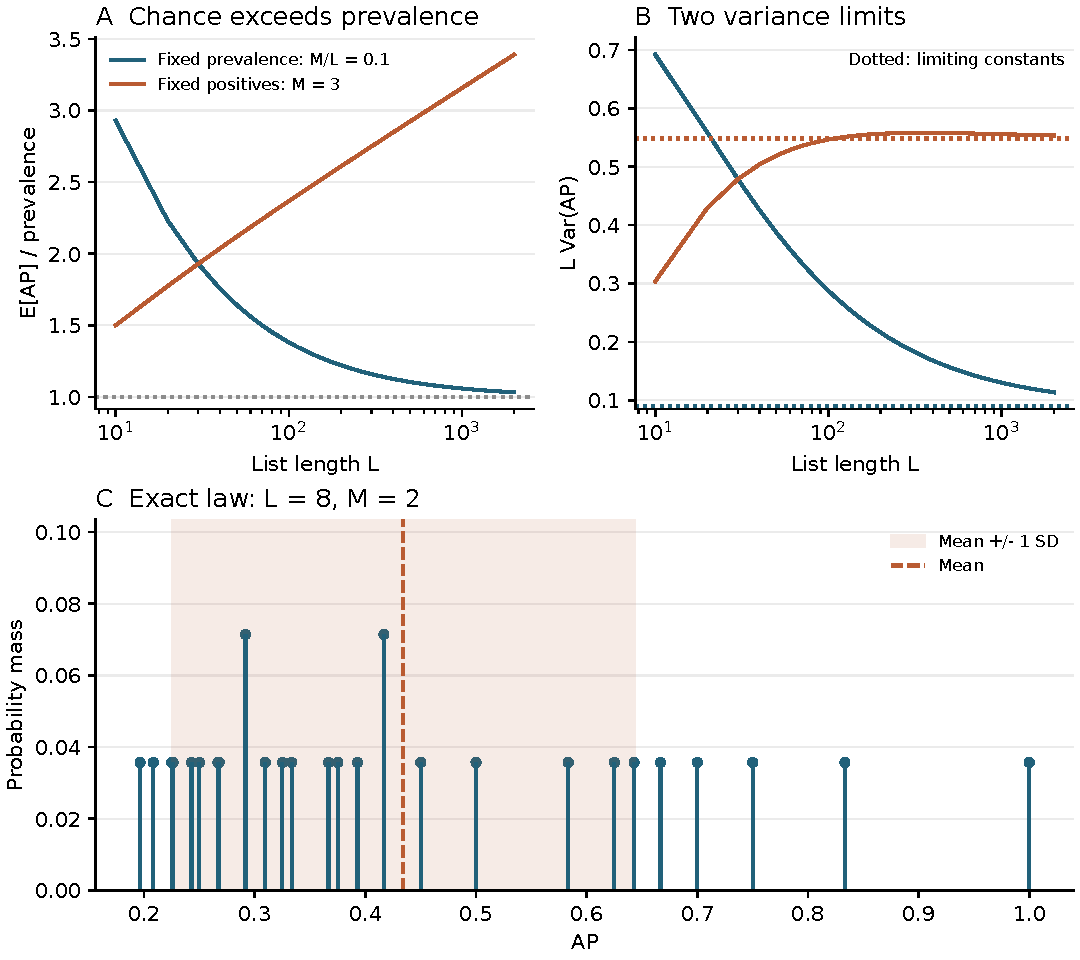
\includegraphics[width=\textwidth]{figures/ap.pdf}
\caption{Exact moments and a discrete AP law.
(A) Mean divided by prevalence for $M/L=0.1$ and for $M=3$.
(B) Variance multiplied by $L$; dotted lines mark the respective limits $0.09$ and $\pi^2/18$.
(C) All 28 label vectors with $L=8$, $M=2$ produce 26 distinct AP values; equal values are combined into probability masses.
The dashed line is the mean, and the shaded band is one standard deviation on either side.
It is not a confidence interval or an interval with a specified coverage probability.}
\label{fig:demo}
\end{figure}

The finite law admits the representation
\[
 \Pr(A=a)=\frac{\#\{R\subseteq\{1,\ldots,L\}:|R|=M,\ A(R)=a\}}{\binom LM}.
\]
The numerator still counts subsets producing a particular atom.
This representation is useful for small cases and verification, but does not supply a compact evaluated expression for general tails.
Nor does it show that no such expression can exist.
Mean and variance alone do not determine these tails or justify a normal approximation.

\section{Formal verification and reproducibility}
The supplement contains the three Lean modules needed for the mean, rank-subset representation, and second moment, together with an audit of the named results.
The pinned toolchain is Lean 4.23.0-rc2, and the dependency revisions are fixed by the Lake manifest.
The expectation theorem is \texttt{expected\_ap\_closed\_form}; the variance theorem is \texttt{varianceAP\_closed\_form}.
Both require $L>1$ and a nonzero positive count.
The second-moment theorem requires only the latter condition, and separate variance theorems cover zero positives, one positive, and all items positive.
All these names are in namespace \texttt{ExpectedAp}.

The atom theorem is stated for rational AP values, with positive count determined by the label vector.
PMF normalization requires $M\le L$.
The eight audited results depend only on propositional extensionality, classical choice, and quotient soundness: \texttt{propext}, \texttt{Classical.choice}, and \texttt{Quot.sound}.
No audited result depends on an admitted-proof or native-computation axiom.
The accompanying verification record gives exact source hashes, theorem assumptions, and commands.
This audit does not certify the Python implementation, asymptotic expansions, or literature comparisons in Lean.

The Python demonstration checks the mean and variance by exhaustive enumeration for every $1\le M\le L\le10$.
An additional check evaluates the four coefficient sums directly and checks symbolic equivalence to the published variance.
The supplement specifies locked Python dependencies, paper compilation, and Lean verification in one reproducible workflow.
No notebook, input dataset, or stochastic simulation is required.

Finally, all moment results here concern the marginal law of one ranking.
They do not imply independence between AP scores from different queries or profiles.
The variance of an average requires covariances unless independence is separately justified.
Dependent mAP models and tail approximations therefore remain outside the scope of this note.

\section*{Acknowledgments}
We appreciate funding from the National Institutes of Health (NIH MIRA R35 GM122547 to AEC).

\paragraph{AI assistance.}
Claude (Anthropic) and Codex (OpenAI) assisted with mathematical exploration, code and Lean proof development, literature comparison, and manuscript drafting and revision.
AI-generated suggestions were evaluated through mathematical review, numerical checks, and Lean verification where applicable.
The authors are responsible for the final content; the scope and limitations of formal verification are described above.

\clearpage
\appendix
\section{Evaluation of the moment sums}\label{app:sums}
Put $X_{ii}=Z_i/i$ and $X_{ik}=Z_iZ_k/k$ for $i<k$.
Call a diagonal term a singleton and an off-diagonal term a pair.
Define
\[
 S_r=\sum_{\substack{i\le k,\ j\le l\\|\{i,k,j,l\}|=r}}\frac1{kl}.
\]
All ranks range from 1 to $L$.
The sum is over ordered pairs of terms, so a product of different terms occurs twice.
Since $Z_i^2=Z_i$, the second moment is $\E[W^2]=\sum_{r=1}^4m_rS_r$.

For one rank, both terms are the same singleton, giving $S_1=H_2$.
For two fixed ranks $a<b$, the two distinct singletons contribute $2/(ab)$, a singleton multiplied by the pair contributes $2/(ab)+2/b^2$, and the pair squared contributes $1/b^2$.
Thus
\begin{align*}
 S_2&=4\sum_{a<b}\frac1{ab}+3\sum_{b=1}^L\frac{b-1}{b^2}\\
 &=2(H^2-H_2)+3(H-H_2)=2H^2+3H-5H_2.
\end{align*}
For three fixed ranks $a<b<c$, a singleton and a disjoint pair contribute $2/(ac)+4/(bc)$.
Two distinct pairs sharing one rank contribute $4/(bc)+2/c^2$.
Their combined weight is therefore $2/(ac)+8/(bc)+2/c^2$.
For each fixed $c$,
\begin{align*}
 \sum_{1\le a<b<c}\frac1{ac}
 &=\frac{(c-1)H_{c-1}-(c-1)}c,\\
 \sum_{1\le a<b<c}\frac1{bc}
 &=\frac{c-1-H_{c-1}}c.
\end{align*}
There are $(c-1)(c-2)/2$ choices of $(a,b)$.
With $H_0=0$, this yields
\[
 S_3=\sum_{c=1}^L\left[\left(2-\frac{10}c\right)H_{c-1}+7-\frac9c+\frac2{c^2}\right].
\]
The summand vanishes at $c=1,2$, as required.
Reversing summation and splitting the harmonic square give
\[
 \sum_{c=1}^LH_{c-1}=LH-L,
 \qquad\sum_{c=1}^L\frac{H_{c-1}}c=\frac{H^2-H_2}2.
\]
Consequently, $S_3=2LH+5L-5H^2-9H+7H_2$.
Every ordered pair of terms has between one and four distinct ranks, and the unrestricted coefficient sum is
\[
 \sum_{r=1}^4S_r=\left(\sum_{k=1}^L\sum_{i=1}^k\frac1k\right)^2=L^2.
\]
Subtracting $S_1,S_2,S_3$ gives
\[
 S_4=L^2-2LH-5L+3H^2+6H-3H_2.
\]
These identities also hold when the corresponding rank sets are empty at small $L$.
They complete the proof of Proposition~\ref{prop:second}.

\section{Variance expansions}\label{app:asymptotic}
For fixed $p\in(0,1)$ and fixed positive integer $r$, expansion of the finite product defining $m_r$ gives
\[
 m_r=p^r-\binom r2\frac{p^{r-1}(1-p)}L+O(L^{-2}).
\]
Equation~\eqref{eq:bias} gives
\[
 \mu_0=p+\frac{(1-p)(H-1)}L+O(H/L^2).
\]
In~\eqref{eq:ew2}, retain $m_4L^2$, $2(m_3-m_4)LH$, and $5(m_3-m_4)L$.
The omitted terms contribute $O(H^2/L^2)$ after division by $M^2=p^2L^2$.
Using $H=O(\log L)$ and $H_2=O(1)$ yields
\begin{align*}
 \E[A^2]&=p^2+\frac{p(1-p)(2H-1)}L+O(H^2/L^2),\\
 \mu_0^2&=p^2+\frac{2p(1-p)(H-1)}L+O(H^2/L^2).
\end{align*}
Subtracting cancels the harmonic terms and proves the fixed-prevalence expansion.
The implicit constants may depend on $p$.

For fixed $M$, instead $m_r=O(L^{-r})$ for $r\le M$ and $m_r=0$ for $r>M$.
The four coefficient sums have orders $1$, $H^2$, $LH$, and $L^2$.
It follows that
\[
 \E[A^2]=\frac{H_2}{ML}+O(H^2/L^2),\qquad
 \mu_0^2=O(H^2/L^2).
\]
Using $H_2=\pi^2/6+O(L^{-1})$ proves the fixed-$M$ limit.

\begin{thebibliography}{9}
\bibitem{zhang} P. Zhang and W. Su.
Statistical inference on recall, precision and average precision under random selection.
In \emph{2012 Ninth International Conference on Fuzzy Systems and Knowledge Discovery}, pp.~1348--1352, 2012.
\href{https://doi.org/10.1109/FSKD.2012.6234049}{doi:10.1109/FSKD.2012.6234049}.
\bibitem{lopes} M. Lopes and G. Bontempi.
On the null distribution of the precision and recall curve.
In \emph{Machine Learning and Knowledge Discovery in Databases}, LNCS 8725, pp.~322--337, 2014.
\href{https://doi.org/10.1007/978-3-662-44851-9_21}{doi:10.1007/978-3-662-44851-9\_21}.
\bibitem{bestgen} Y. Bestgen.
Exact expected average precision of the random baseline for system evaluation.
\emph{Prague Bulletin of Mathematical Linguistics}, 103:131--138, 2015.
\href{https://doi.org/10.1515/pralin-2015-0007}{doi:10.1515/pralin-2015-0007}.
\bibitem{manzhos} T. Manzhos, T. Ianevych, and O. Melnyk.
Average precision at cutoff $k$ under random rankings: expectation and variance.
\emph{Modern Stochastics: Theory and Applications}, 13(3):357--374, 2026.
\href{https://doi.org/10.15559/26-VMSTA298}{doi:10.15559/26-VMSTA298}.
Preprint: \href{https://arxiv.org/abs/2511.02571}{arXiv:2511.02571}, November 2025.
\end{thebibliography}
\end{document}
